
% Sections are a sub-unit
\section{Immune Cell Lineage}

\begin{figure}
    \centering
    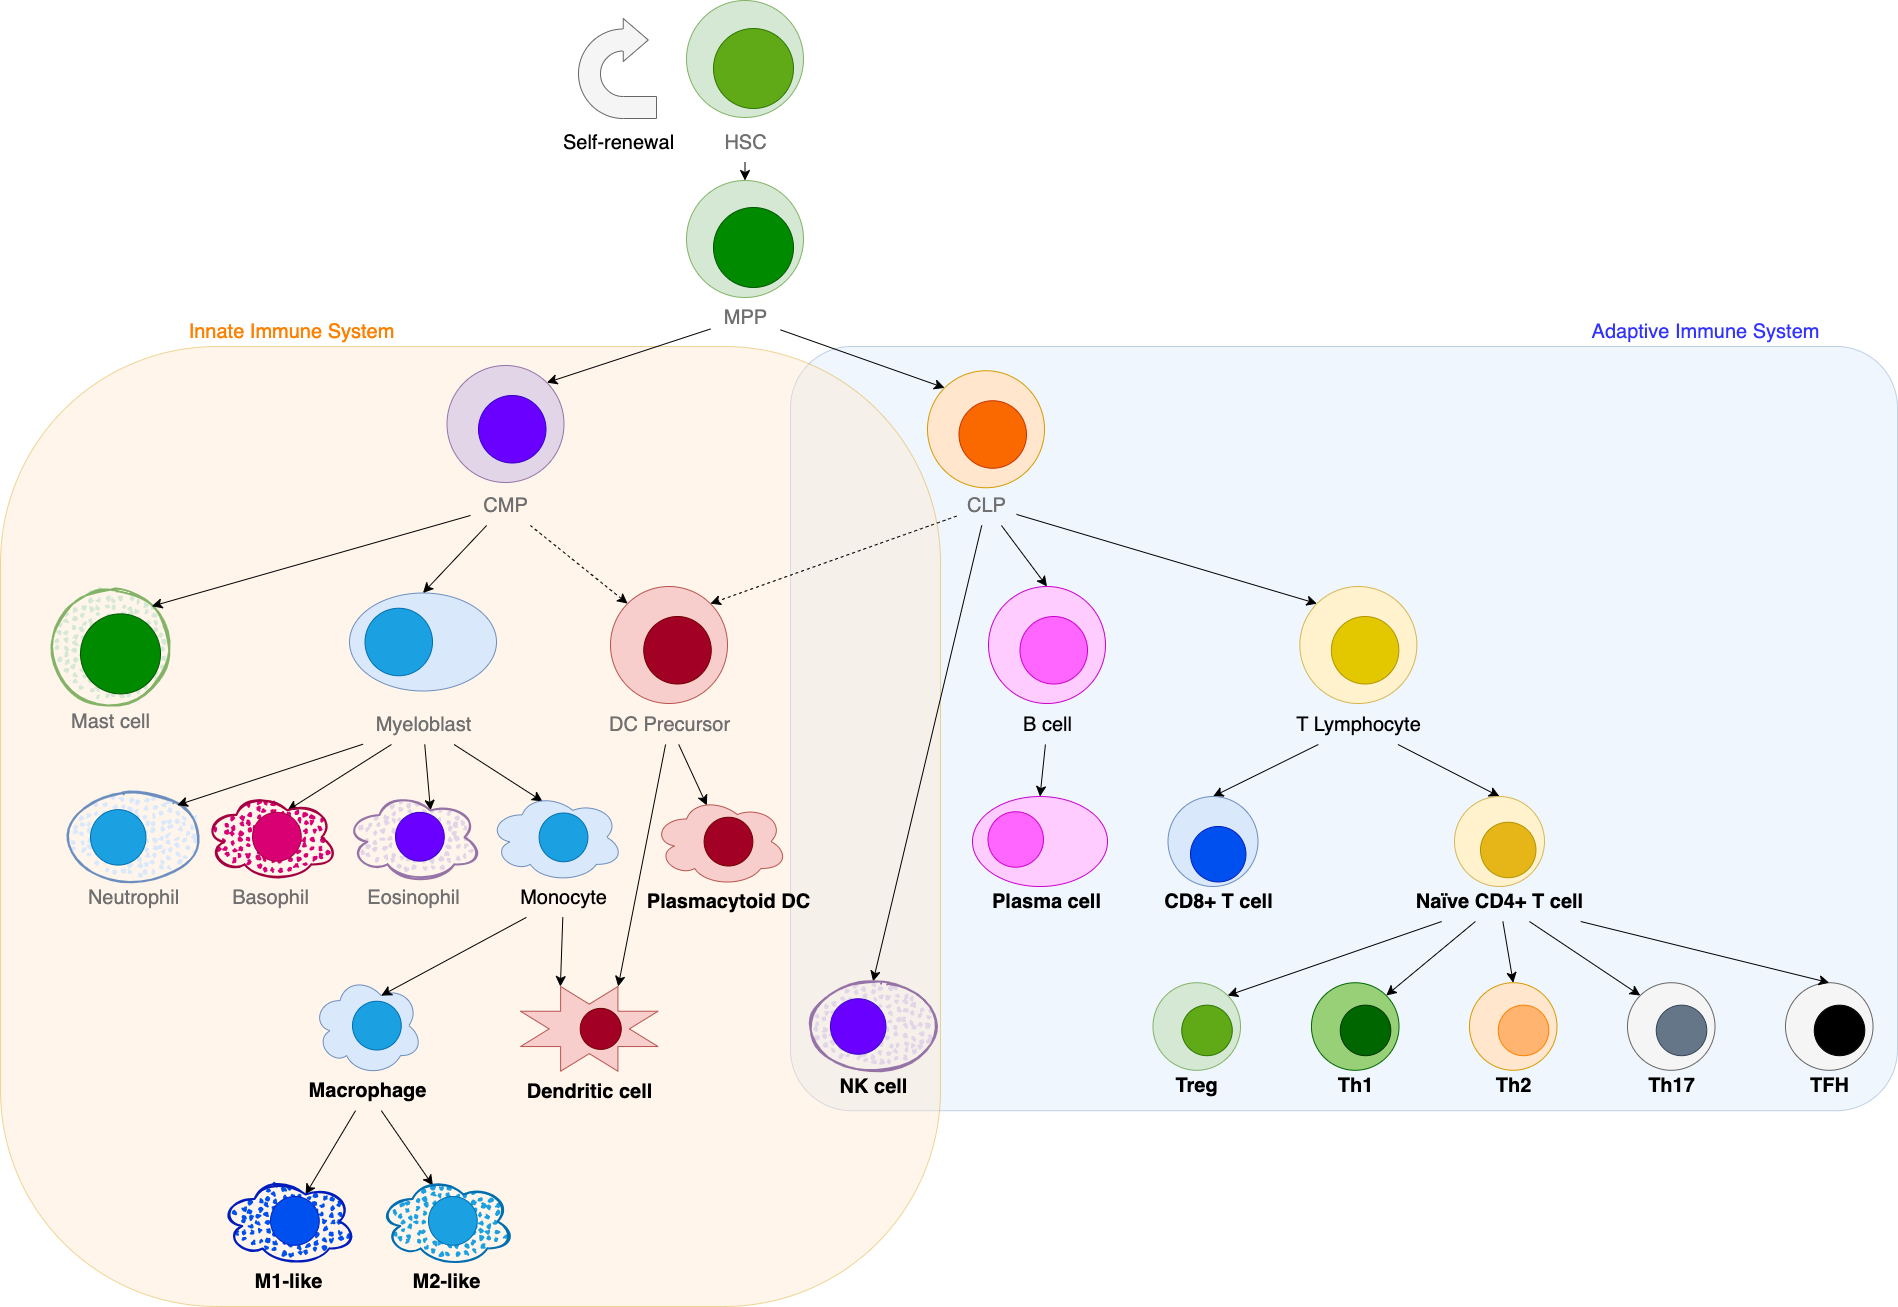
\includegraphics[width=\textwidth]{Figures/immunediff.png}
    \caption{\textbf{Lineage Tree representation of immune cell differentiation} Immune cells are derived from HSCs. HSCs then develop into multipotent progenitors (MPPs) in preparation for further differentiation. MPPs differentiate into common lymphoid and myeloid progenitors (CLPs and CMPs, respectively) before further development into more specified immune cell types within the adaptive and innate immune systems. Cells that are included in peripheral blood mononuclear cells (PBMCs) are in bold.}
    \label{fig:immune-cells}
\end{figure}

The immune system performs a wide range of functions within the body, including defense against pathogens and tumours and maintaining homeostasis of various body systems. In order to perform its role, the immune system relies on the coordinated efforts of complex immune response mechanisms. These mechanisms fall within either the innate immune system or the adaptive immune system and are executed by specialized immune cells each with their own specific role and function. The innate immune system is the body's first line of defense against common microorganisms. Innate immune responses are able to rapidly identify molecular patterns common to microbes and toxins foreign to the host through hard-wired responses encoded within the genes of the host's germ line \cite{immunediff}. For pathogens unable to be fought by the innate immune system, the adaptive immune system takes over by utilizing antigen specific recognition to target specific pathogens. These antigen specific cells are committed to memory through long-lived dormant cells that persist following a pathogen's first offense allowing the adaptive immune system to protect against subsequent reinfections from the same pathogen \cite{immunediff, Janeway2001}. Innate immune cells are comprised of innate lymphocytes such as natural killer (NK) cells and myeloid cells, including eosinophils, neutrophils, basophils, monocytes, and mast cells while adaptive immune cells are primarily made up of B Lymphocytes and T lymphocytes \cite{Klinke2019}.

There are over 80 different identified immune cell subsets each with specialized functions and characterized by specific cellular markers. Despite great heterogeneity amongst the various immune cell subsets, they are all commonly derived from hematopoietic stem cells (HSCs) in bone marrow. Through a multi-step differentiation process, immune cells commit to a cell lineage determined by various external and intrinsic factors including transcriptional reprogramming \cite{Wang2018}. Since the differentiation process contains a number of sequential specialization steps where the immune cells become increasingly distinct, the immune cell landscape is often referred to and depicted as a hierarchical lineage tree \cite{Klinke2019} (Fig. \ref{fig:immune-cells}). 

\subsection{Drivers of Immune Cell Differentiation}

\begin{figure}
    \centering
    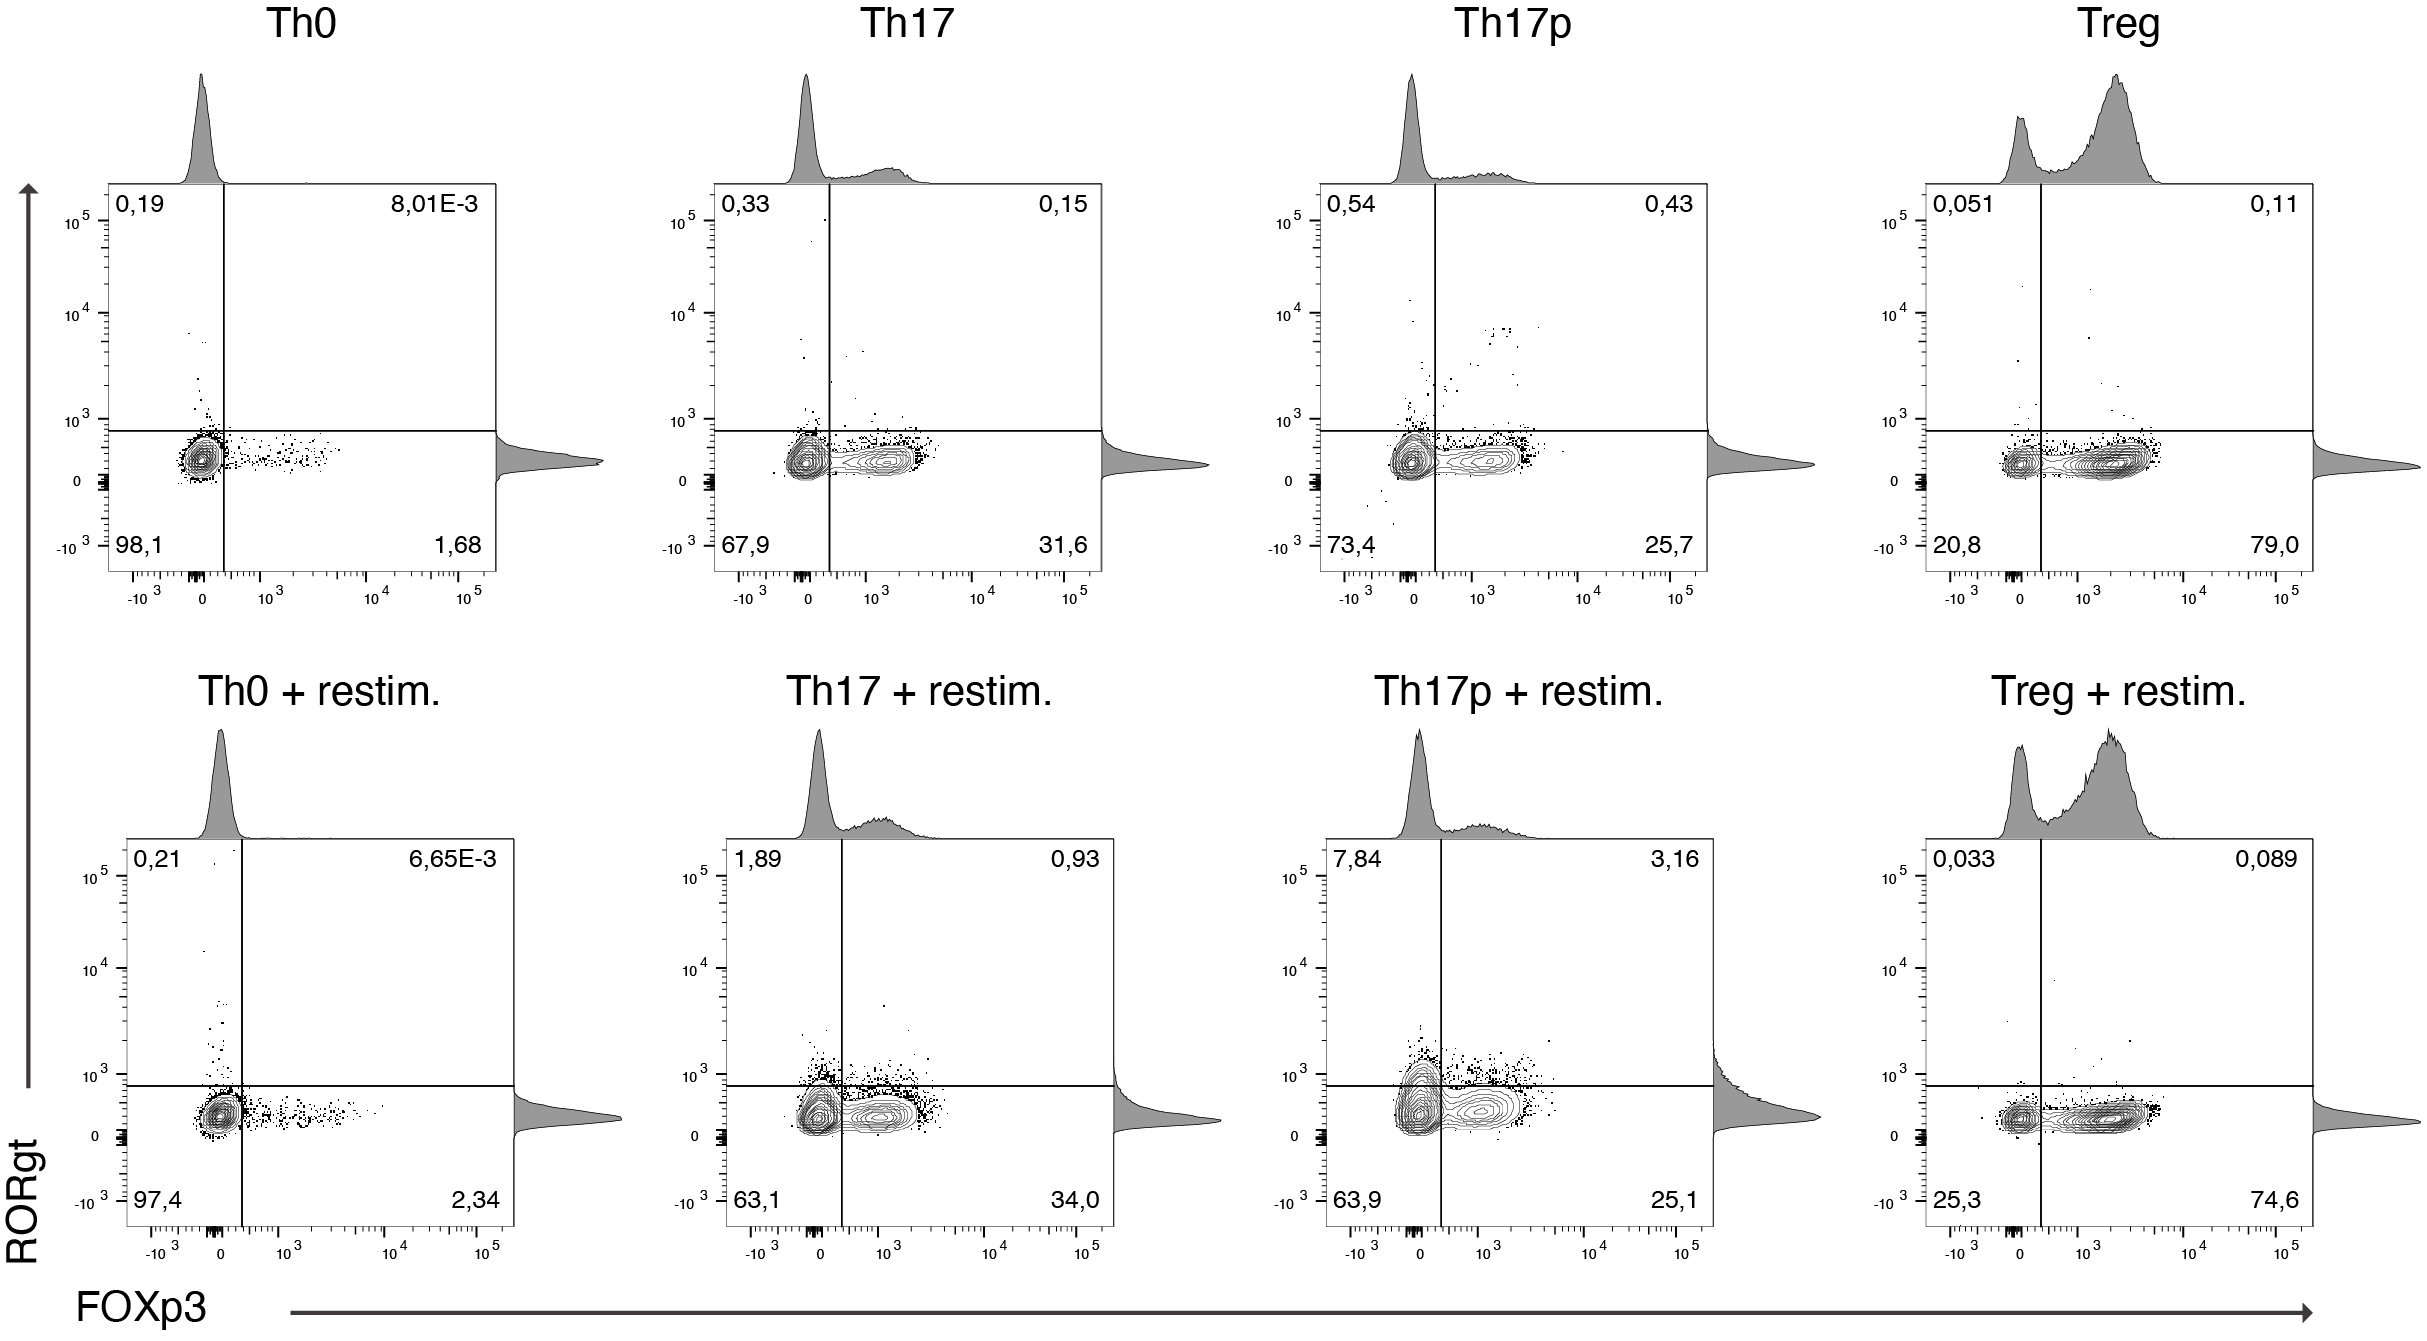
\includegraphics[width=\textwidth]{Figures/FOXp3_vs_RORgt.png}
    \caption{\textbf{\textit{In vitro} polarization of CD4+ T cells results in heterogeneous cell populations} Flow cytometry analysis performed on \textit{in vitro} polarized CD4+ T cells in Th0, Th17, pathogenic Th17 (Th17p), and Treg polarization conditions. Flow plots show protein expression of Foxp3 and Ror$\gamma$t \textemdash markers of Tregs and Th17, respectively \textemdash  in mouse CD4+ T cells.}
    \label{fig:CD4flow}
\end{figure}


\renewcommand{\arraystretch}{1.25}
\begin{sidewaystable}[]
\centering
\scalebox{0.8}{
\begin{tabular}{|c|c|c|c|c|c|c|c|c|c|}
\hline
\multicolumn{10}{|c|}{Treg} \\
 \hline
        Study & $\alpha$ CD3 & $\alpha$ CD28 & IL-2 & TGF-$\beta$ & TNF-$\alpha$ &  $\alpha$ IFN$\gamma$ & $\alpha$ IL-4 & $\alpha$ IL-12 & \textemdash\\
        \hline
        Field 2020 \cite{Field2020} & 5 $\mu$g/mL & 0.5 $\mu$g/mL & 100 U/mL & 5 ng/mL & \textemdash & 10 $\mu$g/mL & 10 $\mu$g/mL & 10 $\mu$g/mL & \textemdash\\
        Yang 2019 \cite{Yang2019} & beads & beads & 50 U/mL & 2 ng/mL & "accordingly" & \textemdash & \textemdash & \textemdash & \textemdash\\
        Xiao 2016 \cite{Xiao2016} & beads & beads & 25 U/mL & 3 ng/mL & \textemdash & \textemdash & \textemdash & \textemdash & \textemdash\\
        Thomas 2012 \cite{Thomas2012} & 1 $\mu$g/mL & 1 $\mu$g/mL & 20 U/mL & 5 ng/mL & \textemdash & \textemdash & \textemdash & \textemdash & \textemdash\\
        Jiang 2018 \cite{Jiang2018} & 5 $\mu$g/mL & 5 $\mu$g/mL & 10 U/mL & 2 ng/mL & \textemdash & \textemdash & \textemdash & \textemdash & \textemdash\\
        Pham 2014 \cite{Pham2014} & 2 $\mu$g/mL & 0.5 $\mu$g/mL & \textemdash & 2 ng/mL & \textemdash & \textemdash & \textemdash & 10 $\mu$g/mL & \textemdash\\
        Wagner 2021 \cite{Wagner2021} & 1 $\mu$g/mL & 1 $\mu$g/mL & \textemdash & 2 ng/mL & \textemdash & \textemdash & \textemdash & \textemdash & \textemdash\\
        Puleston 2021 \cite{Puleston2021} & 5 $\mu$g/mL & 2 $\mu$g/mL & 100 U/mL & 10 ng/mL & \textemdash & 4 $\mu$g/mL & 4 $\mu$g/mL & \textemdash & \textemdash\\
        \hline
 \multicolumn{10}{|c|}{Th17} \\
 \hline
        Study & $\alpha$ CD3 & $\alpha$ CD28 & IL-1$\beta$ & IL-2 & IL-6 & IL-23 & TGF-$\beta$ & $\alpha$ IFN$\gamma$ & $\alpha$ IL-4 \\
        \hline
        Field 2020 \cite{Field2020} & 5 $\mu$g/mL & 0.5 $\mu$g/mL & 10 $\mu$g/mL & 100 U/mL & 10 ng/mL & \textemdash & 5 ng/mL & 10 $\mu$g/mL & 10 $\mu$g/mL\\
        Yang 2019 \cite{Yang2019} & 1 $\mu$g/mL & 1 $\mu$g/mL & \textemdash & \textemdash & 10 ng/mL & \textemdash & 2 ng/mL & 5 $\mu$g/mL & 5 $\mu$g/mL\\ 
        Chen 2017 \cite{Chen2017} & beads & beads & \textemdash & 100 U/mL & 20 ng/mL & \textemdash & 20 ng/mL & \textemdash & \textemdash\\
        Thomas 2012 \cite{Thomas2012} & 1 $\mu$g/mL & 1 $\mu$g/mL & \textemdash & \textemdash & 10 ng/mL & 10 ng/mL & 1 ng/mL & 20 $\mu$g/mL & 20 $\mu$g/mL\\
        Jiang 2018 \cite{Jiang2018} & 5 $\mu$g/mL & 5 $\mu$g/mL & 10 ng/mL & \textemdash & 20 ng/mL & 50 ng/mL & 0.5 ng/mL & \textemdash & \textemdash\\
        Pham 2014 \cite{Pham2014} & 2 $\mu$g/mL & 0.5 $\mu$g/mL & 10 ng/mL & \textemdash & 100 ng/mL & 10 ng/mL & 2 ng/mL & 10 $\mu$g/mL & 10 $\mu$g/mL\\
        Wagner 2021 \cite{Wagner2021} & 1 $\mu$g/mL & 1 $\mu$g/mL & 20 ng/mL & \textemdash & 25 ng/mL & 20 ng/mL & \textemdash & \textemdash & \textemdash\\
        Gaublomme 2015 \cite{Gaublomme2015} & 2 $\mu$g/mL & 2 $\mu$g/mL & 20 ng/mL & \textemdash & 25 ng/mL & 20 ng/mL & 2 ng/mL & \textemdash & \textemdash\\
        Puleston 2021 \cite{Puleston2021} & 5 $\mu$g/mL & 2 $\mu$g/mL & 10 ng/mL & 100 U/mL & 5 ng/mL & \textemdash & 10 ng/mL & 10 $\mu$g/mL & 10 $\mu$g/mL\\
         \hline
    \end{tabular}
}
\caption{\textbf{Table summary of CD4+ polarization conditions} A meta-analysis of various studies with \textit{in vitro} CD4+ subset polarization condition protocols. Included are the polarization conditions for Tregs and Th17s across 10 studies. Units are presented as described in the original studies.}
\label{tab:CD4polarization}
\end{sidewaystable}

The process of immune cell differentiation is driven by cell signaling, a highly variable process influenced by a large number of factors including extracellular environment cytokine presence \cite{Sch_nherr_2000}, epigenetic mechanisms \cite{TURNER2020117}, cellular metabolism \cite{Pearce_2021, Chapman_2017}, transcription factors (TFs) \cite{Liu_2022}, host and host environment, and  microbiome \cite{ter_Horst_2016}. 

The complexity of immune cell differentiation is best exemplified through CD4+ helper T cell polarization. Naïve CD4+ T cells further differentiate into helper T cell subsets marked by distinct gene expression signatures, including cytokine expression, and require the presence of specific extracellular cytokines to polarize \cite{Zhang_2012}. In general, CD4+ T cell populations are heterogeneous following polarization as shown from flow cytometry analysis performed as described in \ref{cha:cd4diff} (Fig. \ref{fig:CD4flow}). Protein expression levels of Foxp3 and Ror$\gamma$t \textemdash regulatory markers of regulatory T cells (Tregs) and Th17 cells, respectively \textemdash are shown \cite{Rudensky_2011, Ivanov_2006}. Both Foxp3 and Ror$\gamma$t are induced in the presence of Tgf-$\beta$ and in the absence of a proinflammatory cytokine, such as IL-6, Foxp3 can inhibit Ror$\gamma$t function to drive towards a Treg phenotype \cite{Ziegler_2009}. The fate of CD4+ T cells is therefore highly influenced by the balance between these two proteins. In the Th17 and pathogenic Th17 (Th17p) polarization conditions without additional restimulation, only a very small subset of cells express Ror$\gamma$t, while a larger subset of cells express Foxp3, suggesting that cells are leaning towards a more suppressive phenotype rather than an effector Th17 phenotype. Cells expressing Ror$\gamma$t and therefore exhibiting a Th17 phenotype are only seen upon restimulation, though the population of suppressive Foxp3+Ror$\gamma$t- cells are still present in the same proportion (Fig.\ref{fig:CD4flow}).

Another factor that contributes to the uncertainty in the differentiation process of immune cells is plasticity between subsets, in the context of CD4+ T cells, it is the ability of a single cell to exhibit features of a number of T cell subsets simultaneously or over time \cite{Geginat_2014}.

A meta-analysis of a number of CD4+ polarization protocols summarized in Table \ref{tab:CD4polarization} and \ref{tab:CD4polarizationSupp} found a lack of consensus between researchers on the necessary extracellular cytokines and their quantities for subset polarization, particularly for Th17 polarization. This demonstrates that CD4+ T cell subset differentiation and immune cell differentiation in general is not entirely understood and there exists the need to further investigate their driving mechanisms and ways to capture the heterogeneous nature of these cell populations in a hierarchical manner. 

\newpage
\section{Pathogenesis of Systemic Lupus Erythematosus}

Systemic Lupus Erythematosus (SLE) is a complex, chronic autoimmune disease that affects approximately 3.17 million adults worldwide \cite{slepath, Tian_2022}. The disease presentation of SLE is highly heterogeneous between individuals and may affect any part of the body, but symptoms typically include fatigue, skin rashes, chronic inflammation, and fever. Many patients suffer from periods of disease exacerbations (flares) where worse or new symptoms are seen in one of more organ systems and a change or increase in treatment is required to suppress the overactive immune response \cite{Adamichou_2017}. Currently, there is no cure for SLE and therapeutic treatments of this disease severely affect the quality of life for patients.

Genetic factors play a crucial role in the development of SLE. About 90\% of SLE cases are female, however this sex difference remains poorly understood \cite{Furst_2012, Nusbaum_2020}. There is also a large discrepancy in the prevalence of SLE between races/ethnic backgrounds. East Asian and Hispanic/South American populations see the highest incidence rates of SLE \cite{Woo_2022}. The heritability of the disease is estimated to be around 44\% \cite{Kuo_2015}, but there has been great difficulty in pinpointing any specific genetic cause of disease manifestation \cite{Ceccarelli_2015}. Currently, there are over 60 confirmed genetic risk loci associated with SLE \cite{TERUEL2016161}. Many of the genes containing these loci are involved with regulatory functions within the innate and adaptive immune system. Genetic variants are suggested to have a regulatory effect on disease pathology since the majority of the SNPs found to be associated with SLE fall within non-coding regions of the gene. Despite the identification of many genetic risk loci, they are only able to explain a small fraction of the heritability of SLE. There are no genetic factors that have been found to be shared between all SLE patients due to the heterogeneous nature of disease manifestation \cite{Ceccarelli_2015}. 

There are a number of environmental factors that have been shown to be significantly associated with the presence of SLE. These factors include exposures such as air pollution, heavy metals, and ultraviolet radiation. Certain lifestyle choices also contribute to the development of SLE including alcohol consumption, cigarette smoking, sleep patterns, socioeconomic factors and stress, and diet and microbiome \cite{Woo_2022}. 

Epigenetic factors, innate and adaptive immunity, and inflammation have also been found to play a role in SLE pathogenesis and exist in the interface between environmental exposures and genetic risk factors and provide potential mechanisms to explain the effect of environmental exposures on disease. \cite{TERUEL2016161, Woo_2022}.


Several different risk factors are hypothesized to be associated with the development of SLE, but a direct cause of SLE remains unclear. The disease mechanism of SLE disease presentation is an area of ongoing investigation, but one known driver is the presence of autoreactive T and B cells, resulting in persistent inflammatory responses in the absence of pathogens. A better understanding of the cellular makeup of circulating immune cells in the body provides further insight into the causal mechanisms in SLE and other autoimmune disorders.

\subsection{Role of T Cells in SLE}

SLE pathogenesis is characterized by the presence of autoantibodies leading to chronic inflammation causing damage to tissues and organs. These autoantibodies are the result of defects in cellular apoptotic debris clearance, pro-inflammatory expression signatures in peripheral lymphocytes, and dysfunctional peripheral tolerance mechanisms \cite{slepath}. 

T cells contribute to SLE pathogenesis through the amplification of inflammation by secretion of pro-inflammatory cytokines. Additionally, the accumulation of autoreactive memory T cells results in sustaining disease over time.

CD4+ helper T cells signal to B cells through the production of cytokines. Abnormalities in the T cell receptor (TCR) leads to increased stimulation and results in aberrant activation of T cells \cite{Moulton_2015}. SLE patients have an imbalance of CD4+ T cell subsets. In peripheral blood CD4+ T cell populations, pro-inflammatory Th17s are overabundant, while suppressive Tregs are under-represented. As a result, there is an increased prevalence of the pro-inflammatory signaling cytokines IL-6 and IL-17 \cite{Talaat_2015}. Additionally, aberrant activation of PI3K/AKT/mTOR signal transduction leads to an increased accumulation of effector/memory T cells due to a resistance to activation-induced cell death \cite{Su_rez_Fueyo_2011}. Meanwhile, dysfunction in CD8+ T cells in SLE results in dampended cytotoxicity and results in increased risk of infection, potentially triggering autoimmunity \cite{Gravano_2013}. 

The significant role that T cells play in SLE pathogenesis, coupled with the lack of understanding behind the genetic drivers of SLE and the complex mechanisms of immune cell differentiation inspires the need to further investigate genomic mechanisms in immune cell subsets in patients with SLE.

\newpage
\section{Latent Representations of Biological Data} 

With the recent advancements of high-throughput screening (HTS) technologies, specifically single-cell RNA sequencing (scRNA-seq), knowledge of the molecular profiles of specific cell types has expanded. Since scRNA-seq data is high-dimensional, often capturing expression of tens of thousands of genes across thousands of cells, scalable and interpretable computational methods are necessary to perform sophisticated analysis of the data in order to uncover biological insights. One branch of these methods focuses on representing scRNA-seq data in a lower dimension latent space in a meaningful and interpretable way. Latent representations of biological data allows for further downstream analysis, such as cellular deconvolution using unsupervised clustering techniques \cite{Luecken_2019}. 

A key challenge in latent embedding of biological data is the inability to produce biologically interpretable results. Therefore extracting meaning from the data requires backfilling of information through manual annotation and analysis \cite{Kiselev_2019}.

\subsection{Deep-learning Methods for Biological Data} 

As datasets become increasingly large in the number of samples as well as dimensionality, there has been a shift towards deep-learning methods which are scalable and out-perform linear methods such as the iterative Harmony algorithm \cite{korsunsky2019fast} and non-negative matrix factorization (NMF) based methods such as LIGER \cite{liu2020jointly}.

Deep-learning based approaches for scRNA-seq most commonly use autoencoders, a type of artificial neural network, as a means to project high-dimensional data onto a low-dimensional latent space \cite{tschannen2018recent}. A number of recent methods utilize a variational autoencoder (VAE) \cite{Kingma2013-if}, a Bayesian method that relies on stochastic variational inference to efficiently scale to large datasets. These methods include single-cell variational inference (\texttt{scVI}) \cite{scvi} and single-cell VAE (\texttt{scVAE}) \cite{gronbech2020scvae}, the latter of which extends the VAE framework by using a Gaussian-mixture model as the prior distribution for latent variables over a Gaussian prior to learn cell clusters through a categorical latent variable.

Single-cell Embedded Topic Model (\texttt{scETM}) \cite{scETM} and Bayesian latent topic analysis with sparse association matrix (\texttt{BALSAM}) \cite{ZHANG2023100388}  are methods that make use of an embedded topic model (ETM) framework \cite{etm1}, an extension of VAE. In these methods, neural networks are used to encode scRNA-seq data into a latent topic space, while a generalized linear model (GLM) is used to decode latent embeddings back to the original gene expression space. As a result, these methods are able to simultaneously learn the parameters of the encoder neural networks and topic specific gene embeddings to create a highly interpretable latent space. 

\subsection{Methods to Model Cellular Hierarchies}

It has been suggested to use a tree-based reference structure to represent cell types as opposed to an atlas or periodic table-like classification system in order to better capture relationships between cell types \cite{treeref}. 

Therefore, a method that can embed scRNA-seq data in an interpretable latent space while learning a hierarchical tree-structure of data has the potential effectively identify cell clusters while providing insights into cellular relationships.

Hierarchical extensions to the topic modeling framework have been proposed where latent topics exist as nodes that lie in a tree structure. These methods include hierarchical latent Dirichlet allocation (\texttt{hLDA}) \cite{hlda} and tree-structured neural topic model (\texttt{TSNTM}) \cite{tree_etm}. \texttt{hLDA} uses a latent Dirichlet allocation (LDA) approach to represent topics in a hierarchical structure informed by a nested Chinese restaurant process prior. \texttt{TSNTM} makes use of autoencoding variational Bayes to efficiently construct a tree-structured latent topic space. Since the latent topic tree structures in these methods exist in an infinite tree space, meaning each node can have infinite child nodes, these models rely on Markov Chain Monte Carlo (MCMC) algorithms in order to simulate models over super-exponential space. Despite theoretical guarantees, these methods were not suitable for the purposes of scRNA-seq data due to the size of the data and the computational complexity associated with learning the topic tree structure. 

Another approach to model hierarchical representations of scRNA-seq data is to do \textit{post-hoc} construction of the tree-structured relationships between cells. \texttt{treeArches} \cite{sc_hier} aims to construct and extend a cell reference atlas and corresponding hierarchical classifier, relying on prior information from an existing cell atlas. \texttt{cellTree} infers tree-structured relationship hierarchies between individual cells based upon LDA latent representations and minimum spanning trees to construct the tree structure. These methods construct their relevant cellular tree representations after estimating their latent representations rather than learning the cellular hierarchies simultaneously with their latent representation. Additionally, \texttt{cellTree} only constructs the direct hierarchical relationships between individual cells, differing from the other modeling approaches which aim to define relationships between cell features through topics in order to represent hierarchical relationships.

\newpage
\section{Thesis Objectives and Hypothesis}
\subsection{Summary of rationale}

Immune cell differentiation is a complex biological process that remains an area for further investigation. The various immune cell subsets originate from a common HSC progenitor and follow a series of branching differentiation steps to reach maturity. As immune cells develop, they become more highly specific in cell features and function, resulting in greater dissimilarity with other immune subsets. The process results in a lineage tree structure between immune cell subsets where cells share hierarchical relationships with one another. Tree-structured latent modeling of HTS data, specifically scRNA-seq, has the potential to uncover insights into the cellular differentiation process, hierarchical relationships between immune cell subsets, and their shared and differing cellular features. Though a number of statistical latent models of scRNA-seq data exist, an efficient and effective tree-structured model for this purpose has yet to be shown.

Applications of such a model may also provide biological insights on the pathogenesis of disease driven by immune dysregulation such as SLE. SLE is a complex autoimmune disease that is characterized by chronic autoinflammation in one or many organ systems. One mechanism driving this autoinflammation is aberrant function and imbalance of peripheral blood lymphocytes. Though SLE is a heritable disease and through genome-wide association studies (GWAS) a number of risk loci have been identified, genetic mechanisms driving disease presentation are not well understood. 

\subsection{Thesis Aims and Outline}

In the work presented in this thesis, there are two main research aims that are addressed. 

First, I aim to develop a tree-structured topic model to represent immune cell subsets and their hierarchical relationships through shared and differing cellular features. In order for this model to be effective for these purposes and provide biological insight, I bear in mind the efficiency and interpretability of methods used. The second aim of this thesis is to apply the developed model to a scRNA-seq dataset from individuals with varying SLE disease conditions to show pathological differences in immune cell composition and identify specific genomic features that may play a role in SLE pathogenesis.

In Chapter \ref{cha:larch}, I propose \texttt{LaRCH} (\underline{La}tent \underline{R}epresentation of \underline{C}ellular \underline{H}ierarchies), a neural topic model with a underlying tree-structure representation of latent topics. This model is based on an ETM framework which allows for highly interpretable topic specific gene embeddings. Autoencoding variational Bayes is used to train the model to ensure computational efficiency. To demonstrate the efficacy of this model, I train LaRCH on a realistic simulated scRNA-seq dataset of immune cell subsets. Using this model I am able to reconstruct cellular hierarchies from their latent topic representations and perform further downstream analysis.

Chapter \ref{cha:sle} of this thesis shows the application of the LaRCH model on a large scRNA-seq dataset of PBMC samples from individuals with varying SLE disease statuses. I demonstrate the ability for LaRCH to deconvolve immune cell subtypes. Then through disease stratified analysis, I identify disease dependent differences in cell-type composition and cellular features. The interpretable model features of LaRCH are used to assign biological meaning to the latent topic space and identify potential genetic drivers of SLE disease mechanisms that inspire further experimental investigation.
